% 
% Permission is granted to copy, distribute and/or modify this document
% under the terms of the GNU Free Documentation License, Version 1.2
% or any later version published by the Free Software Foundation;
% with no Invariant Sections, no Front-Cover Texts, and no Back-Cover
% Texts.  A copy of the license is included in the section entitled "GNU
% Free Documentation License".

\documentclass[11pt]{article}

\usepackage{OTSVM_Documentation}
\usepackage{Math_Notations}

\makeindex

\begin{document}

\thispagestyle{empty}

% 
% Permission is granted to copy, distribute and/or modify this document
% under the terms of the GNU Free Documentation License, Version 1.2
% or any later version published by the Free Software Foundation;
% with no Invariant Sections, no Front-Cover Texts, and no Back-Cover
% Texts.  A copy of the license is included in the section entitled "GNU
% Free Documentation License".
\vspace*{2cm}

\begin{center}
  {\huge \bf Documentation of the OPENTURNS SVM module}

  \vspace{200pt}
  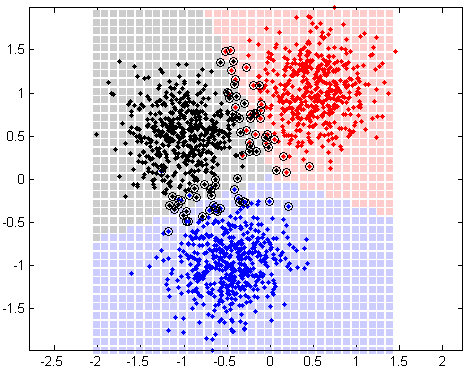
\includegraphics[width=200pt]{logoOTSVM.png}
 
\end{center}



\newpage
%  
%  Permission is granted to copy, distribute and/or modify this document
%  under the terms of the GNU Free Documentation License, Version 1.2
%  or any later version published by the Free Software Foundation;
%  with no Invariant Sections, no Front-Cover Texts, and no Back-Cover
%  Texts.  A copy of the license is included in the section entitled "GNU
%  Free Documentation License".
\vspace{0.5in}
\begin{center}
\vspace{0.3in}
\emph{\fontshape{sc} Abstract}
\vspace{0.5in}
\end{center}

The purpose of this document is to present the OpenTURNS SVM module, which enables to realize support vector regression and classification with Libsvm and to manipualte results with OpenTURNS.

It offers to the user the ability to:
\begin{itemize}
 \item define a regression or a classification problem and solve it with Libsvm
 \item build OpenTURNS objects from Libsvm models
 \item extract metamodels of Libsvm as OpenTURNS metamodels
\end{itemize}


This document is organised according to the Open TURNS documentation :
\begin{itemize}
\item a \itshape{Reference Guide} which gives some theoretical basis on support vector regression.
\item a \itshape{Use cases Guide} which details scripts in python (the Textual Interface langage of Open TURNS) and helps the User to learn as quickly as possible the manipulation of the $otsvm$ module.
\item the \itshape{User Manual} which details the $otsvm$ objects and give the list of their methods.
\end{itemize}


\tableofcontents
\newpage
% 
% Permission is granted to copy, distribute and/or modify this document
% under the terms of the GNU Free Documentation License, Version 1.2
% or any later version published by the Free Software Foundation;
% with no Invariant Sections, no Front-Cover Texts, and no Back-Cover
% Texts.  A copy of the license is included in the section entitled "GNU
% Free Documentation License".




%%%%%%%%%%%%%%%%%%%%%%%%%%%%%%%%%%%%%%%%%%%%%%%%%%%%%%%%%%%%%%%%%%%%%%%%%%%%%%%%%%%%%%%%%% 
\section{Reference Guide}

The Libsvm library provides efficient algorithms to produce a model by Support Vector Machine.

\subsection{Introduction to support vector machine}

A support vector machine is a concept in statistics and computer science for a set of related supervised learning methods that analyze data and recognize patterns, used for classification and regression analysis. 
The standard SVM takes a set of input data and predicts, for each given input, which of two possible classes forms the input. Given a set of training examples, each marked as belonging to one of two categories, a SVM
training algorithm builds a model that assigns new examples into one category or the other.\\

More formally, a SVM constructs a hyperplane in a high or infinite-dimensional space, which can be used for classification or regression. A good separation is acheived by the hyperplane that 
has the largest distance to the nearest training data point of any class.\\

Whereas the original problem may be stated in a finite dimensional space, it often happens that the sets to discriminate are not linearly separable in that space. For this reason,
it was proposed that the original finite-dimensional space be mapped into a much higher-dimensional space, presumably making the separation easier in that space. To keep the computational load reasonable, the mappings used by SVM schemes are 
designed to ensure that dot products may be computed easily in terms of the variables in the original space, by defining them in terms of a kernel function $K(x,y)$ selected to suit the problem.

\subsection{Linear SVM}

Given some training data $D$, a set of n points of the form \[D\ =\ \{(x_{i},y_{i})\ |\ x_{i} \in \mathbb{R}^{p},\ y_{i} \in \{-1,1\}\}^{n}_{i=1}\] where the \begin{math}y_{i}\end{math}
is either 1 or -1, indicating the class to which the point \begin{math}x_{i}\end{math} belongs. Each \begin{math}x_{i}\end{math} is a p-dimensional real vector. 
We want to find the maximum-margin hyperplane that divides the points having \begin{math}y_{i}=1\end{math} from those having \begin{math}y_{i}=-1\end{math}.


Any hyperplane can be written as the set of points \begin{math}x\end{math} satisfying \[w \cdot x - b = 0\] where \begin{math}\cdot\end{math} denotes the dot product and \begin{math}w\end{math} the normal vector
to the hyperplane. We want to choose the \begin{math}w\end{math} and \begin{math}b\end{math} to maximize the margin, or distance between the parallel hyperplanes that are as far apart as possible while still separating the data. These hyperplanes can be
described by the equations \[w \cdot x - b = 1\] \[and\] \[w \cdot x - b = -1\]
The distance between these two hyperplanes is \begin{math}\frac{2}{||w||}\end{math}, so we want to minimize \begin{math}||w||\end{math}. As we also have to prevent data points from falling into the margin, we add the following constraint : for each $i$ either
\begin{equation}y_{i}(w \cdot x_{i} - b)\geq 1\quad for\ all\ 1\leq i\leq n\end{equation}
\newpage
So we get the optimization problem :

\[Min\ ||w||\]
\[subject\ to\ ( for\ any\ i=1,...,n )\] 
\[y_{i}(w \cdot x_{i} - b)\geq 1\]

\subsubsection{Primal form}

The optimization problem presented in the preceding section is difficult to solve because it depends on \begin{math}||w||\end{math}, which involves a square root. It is possible to alter the equation by substituing \begin{math}||w||\end{math} with \begin{math}\frac{1}{2}||w||^{2}\end{math}
without changing the solution. This is a quadratic programming optimization problem :

\[Min\ \frac{1}{2}||w||^{2}\]
\[subject\ to\ ( for\ any\ i=1,...,n )\]
\[y_{i}(w \cdot x_{i} - b)\geq 1\]

By introducing Lagrange multipliers $\alpha$, the previous constrained problem can be expressed as \[\underset{w,b}{\text{min}}\ \underset{\alpha \geq 0}{\text{max}}\{\frac{1}{2}||w||^{2}-\sum_{i=1}^n \alpha_{i}[y_{i}(w \cdot x_{i} - b)-1]\}\]

This problem can now be solved by standard quadratic programming techniques and programs. The stationary Karush-Kuhn-Tucker condition implies that the solution can be expressed as a linear combination of the training vectors \[w = \sum_{i=1}^n \alpha_i y_i x_i\] 

Only a few $\alpha_i$ will be greater than zero. The corresponding $x_i$ are exactly the support vectors, which lie on the margin and satisfy \begin{math}y_i (w\cdot x_i -b)=1\end{math}.

\subsubsection{Dual form}

Using the fact that \begin{math}||w||^2 = w \cdot w \end{math} and substituing \begin{math} w = \sum_{i=1}^n \alpha_i x_i y_i \end{math}, one can show that the dual of the SVM reduces to the following
optimization problem :


\[Max\ L(\alpha) = \sum_{i=1}^n \alpha_i - \frac{1}{2} \sum_{i,j} \alpha_i \alpha_j y_i y_j x_i^T x_j = \sum_{i=1}^n \alpha_i - \frac{1}{2} \sum_{i,j} \alpha_i \alpha_j y_i y_j k(x_i,x_j)\] 

\[subject\ to\ ( for\ any\ i = 1,...,n  )\]
\[\alpha_i \geq 0\]

\[and\ to\ the\ constraint\ from\ the\ minimization\ in\ b\]
\[\sum_{i=1}^n \alpha_i y_i =0\]


$w$ can be computed thanks to the $\alpha$ terms : \[w=\sum_i \alpha_i y_i x_i\]


\subsection{Soft margin}

If there exists no hyperplane that can split the "yes" and "no" examples, the soft margin method will choose a hyperplane that splits the examples as cleanly as possible, while still maximizing the distance to the nearest cleanly split examples. The method introduces slack variables, $\xi_i$, which measure the degree of misclassification of the data $x_i$
\[y_i(w \cdot x_i - b) \geq 1 - \xi_i \quad 1 \leq i \leq n\]
The objective function is then increased by a function which penalizes non-zero $\xi_i$ and the optimization becomes a trade off between a large margin and a small error penalty. If the penalty function is linear, the optimization problem becomes : 
\[\underset{w,b,\xi}{\text{min}}\{\frac{1}{2} ||w||^2 + C\sum_{i=1}^n \xi_i \}\]
\begin{center}subject to (for any $i=1,...,n$)\end{center}
\[y_i ( w \cdot x_i - b) \geq 1 - \xi_i \quad \xi_i \geq 0\]

This constaint with the objective of minimizing $||w||$ can be solved using Lagrange multipliers as done above. One has then to solve the problem :
\[\underset{w,b,\xi}{\text{min}}\ \underset{\alpha,\beta}{\text{max}}\{\frac{1}{2} ||w||^2 + C\sum_{i=1}^n \xi_i - \sum_{i=1}^n \alpha_i[y_i(w \cdot x_i - b)-1 +\xi_i]- \sum_{i=1}^n \beta_i\xi_i \} \] 
\begin{center} with $\alpha_i , \beta_i \geq 0$ \end{center}

The dual form becomes : 
\[\underset{\alpha_i}{\text{max}}\ \{L(\alpha) = \sum_{i=1}^n \alpha_i - \frac{1}{2} \sum_{i,j} \alpha_i \alpha_j y_i y_j k(x_i,x_j)\}\]
\begin{center} subject to ( for any $i=1,...,n$) \end{center}
\[0 \leq \alpha_i \leq C\]
\begin{center} and \end{center}
\[\sum_{i=1}^n \alpha_i y_i = 0\]

\subsection{Nonlinear SVM}

The algorithm is formally similar, except that every dot product is replaced by a nonlinear kernel function. This allows the algorithm to fit the maximum-margin hyperplane in a transformed feature space.
The transformation may be nonlinear and the transformed space high dimensional, thus though the classifier is a hyperplane in the high-dimensional feature space, it may be nonlinear in the original input space.

Some common kernels include : 
\begin{itemize}
 \item Polynomial : $k(x_i,x_j)=(x_i\cdot x_j+c)^d$
 \item Gaussian Radial Basis Function : $k(x_i,x_j)=exp(-\gamma ||x_i-x_j||^2)$
 \item Hyperbolic tangent : $k(x_i,x_j)=tanh(\gamma x_i\cdot x_j + c)$
\end{itemize}
The kernel is related to the transform $\varphi(x_i)$ by the equation $k(x_i,x_j)=\varphi(x_i)\cdot\varphi(x_j)$. The value $w$ is also in the transformed space, with $w=\sum_i\alpha_i y_i\varphi(x_i)$.\\

The effectiveness of SVM depends on the selection of kernel, the kernel's parameters, and soft margin parameter C. A common choice is a Gaussian kernel, which has a single parameter $\gamma$. Best combination of
C and $\gamma$ is selected by a grid search with exponentially growing sequences of C and $\gamma$. Each combination of parameter choices is checked using cross validation, and the parameters with best cross-validation accuracy are picked. 
The final model, which is used for testing and for classifying data, is then trained on the whole training set using the selected parameters.

\subsection{Classification}

Given training vectors $x_i$ in two classes and a vector $y\in{-1,1}$, C-SVC ( the algorithm that we use for classification) solves the following dual problem :
\[min_{\alpha} \frac{1}{2} \alpha^TQ\alpha-e^T\alpha\]
\[0\leq \alpha_i \leq C\]
\[y^T\alpha=0\]
where e is the vector of all ones, $C>0$ is the upper bound, Q is an l by l positive semidefinite matrix $Q_{ij}=y_iy_jK(x_i,x_j)$ and $K(x_i,x_j)$ is the kernel. The decision function is 
\[sign(\sum_{i=1}^l y_i\alpha_iK(x_i,x)+b)\]

For some classification problems, numbers of data in different classes are unbalanced. We can use different penalty parameters in the SVM formulation, the dual of C-SVC becomes :
\[min_{\alpha} \frac{1}{2} \alpha^TQ\alpha-e^T\alpha\]
\[0\leq \alpha_i \leq C_+,\ if\ y_i=1\]
\[0\leq \alpha_i \leq C_-,\ if\ y_i=-1\]
\[y^T\alpha=0\]

where $C_+$ and $C_-$ depending on $y_i$ and $y_j$ and of weights that we can fix for each class.

\subsection{Regression }
Up to now, we presented SVM for classification. We can use too for Regression. This is similar to the nonlinear case. We replace the soft margin by 
a $\varepsilon$-insensitive loss function which is defined like:
\[|y-f(x)|_\varepsilon = max(0,|y-f(x)|-\varepsilon)\]
where f(x) is the loss function and $\varepsilon$ a precision parameter.

We get this optimization problem if we introduce the slack variables $\xi\ and\ \xi_i$:
\[min_w \{\frac{||w||^2}{2}+C\sum_{i=1}^n(\xi_i+\xi_i^*) \}\]
\begin{center}subject to (for any $i=1,...,n$)\end{center}
\[l_i-wx_i+b\leq \varepsilon+\xi_i\]
\[wx_i-b-l_i\leq \varepsilon +\xi_i^*\]
\[\xi_i,\xi_i^* \geq 0\]
with C which is a control parameter like in soft margin. 

To solve this problem, we introduce a new time Lagrange multipliers and we will get this regression function :
\[f(x)=\sum_{i=1}^n(\alpha_i-\alpha_i^*)K(x_i,x)-b\]


 



\newpage
% 
% Permission is granted to copy, distribute and/or modify this document
% under the terms of the GNU Free Documentation License, Version 1.2
% or any later version published by the Free Software Foundation;
% with no Invariant Sections, no Front-Cover Texts, and no Back-Cover
% Texts.  A copy of the license is included in the section entitled "GNU
% Free Documentation License".




%%%%%%%%%%%%%%%%%%%%%%%%%%%%%%%%%%%%%%%%%%%%%%%%%%%%%%%%%%%%%%%%%%%%%%%%%%%%%%%%%%%%%%%%%% 
\section{Use Cases Guide}

This section presents the main functionalities of the module $otsvm$ in their context.



%%%%%%%%%%%%%%%%%%%%%%%%%%%%%%%%%%%%%%%%%%%%%%%%%%%%%%%%%%%%%%
\subsection{Which python modules to import ?}

In order to use the functionalities described in this documentation, it is necessary to import  : 
\begin{itemize}
   \item the openturns python module which gives access to the OpenTURNS functionalities.
   \item the $otsvm$ module which links the $openturns$ functionalities.
\end{itemize}

Python  script for this use case :
\begin{lstlisting}
# Load OpenTURNS 
from openturns import *
#Load the svm module
from otsvm import *
\end{lstlisting}

\subsection{UC : creation of a SVM regression algorithm}

The objective of this Use Case is to create a SVM Regression algorithm in order to create a metamodel.


Otsvm enables :

\begin{itemize}
 \item to set lists of tradeoff factors and kernel parameter with the methods setTradeoffFactor, setKernelParameter.
 \item to select the kernel type in this list : Linear Kernel, Polynomial Kernel, Sigmoid Kernel, RBF kernel.
 \item to compute the algorithm on an input and output samples.
 \item to compute the algorithm on an experiment plane and a function.
 \item to compute the algorithm on an input and output samples and an isoprobabilistic distribution.
\end{itemize}

We recommend for users to use the RBF Kernel ( the gaussian kernel ). Moreover, it is important to understand that the selection of parameters ( kernel parameter and tradeoff factor ) is primary. If you don't know 
what to take as parameters, you must take a wide range values, for example $tradeoff \in \{10^-5,10^-3,10^-1...10^3 \}$ $kernel\ parameter \in \{10^-15, 10^-13...,10^3 \}$. Normally, the algorithm always converges, but this can take a long while, mostly if you have a lot of parameters to test.\\

Python script for this UseCase :
\begin{lstlisting}
#create a function, here we create the Sobol function
dimension = 3
meanTh = 1.0
a = NumericalPoint(dimension)
inputVariables = Description(dimension)
outputVariables = Description(1)
outputVariables[0] = "y"
formula = Description(1)
formula[0] = "1.0"
covTh = 1.0
for i in range(dimension):
  a[i] = 0.5*i
  covTh = covTh * (1.0 + 1.0 / (3.0 * (1.0 + a[i])**2))
  inputVariables[i] = "xi" + str(i)
  formula[0] = formula[0] + " * ((abs(4.0 * xi" +str(i) + " -2.0) + " + 
  str(a[i]) + ") / (1.0 + " + str(a[i]) + "))"
covTh = covTh -1.0
model = NumericalMathFunction(inputVariables, outputVariables, formula)

#create the input distribution
RandomGenerator.SetSeed(0)
marginals = DistributionCollection(dimension)
for i in range(dimension):
  marginals[i] = Uniform(0.0, 1.0)
distribution = ComposedDistribution(marginals)

#create lists of kernel parameters and tradeoff factors
tradeoff = NumericalPoint([0.01,0.1,1,10,100,1000])
kernel = NumericalPoint([0.001,0.01,0.1,1,10,100])

#first example : create the problem with an input and output samples:
#first, we create samples
dataIn = distribution.getNumericalSample(250)
dataOut = model(dataIn)
#second, we create our svm regression object, we must select the third parameter 
#in an enumerate in the list { NormalRBF, Linear, Sigmoid, Polynomial }
Regression = SVMRegression(dataIn, dataOut, LibSVM.NormalRBF)
#third, we set kernel parameter and tradeoff factor
Regression.setTradeoffFactor(tradeoff)
Regression.setKernelParameter(kernel)
# Perform the algorithm
Regression.run()
# Stream out the results
SVMRegressionResult = Regression.getResult()
# get the residual error
residual = result.getResiduals()
# get the relative error
relativeError = result.getRelativeErrors()

#second example : create the problem with an experiment plane:
#first, we create the plane
myPlane = MonteCarloExperiment(distribution, 250)
myExperiment = Experiment(myPlane, "example")
#second, we create our svm regression object, the first parameter is the function
Regression2 = SVMRegression(model, myExperiment, 
LibSVM.Linear)
#third, we set kernel parameter and tradeoff factor
Regression2.setTradeoffFactor(tradeoff)
Regression2.setKernelParameter(kernel)
# Perform the algorithm
Regression2.run()
# Stream out the results
SVMRegressionResult = Regression2.getResult()
# get the residual error
residual = result.getResiduals()
# get the relative error
relativeError = result.getRelativeErrors()

#third example : create the problem with an isoprobabilistic distribution
#first, we create our distribution
marginals = DistributionCollection(dimension)
for i in range(dimension):
  marginals[i] = Uniform(0.0, 1.0)
distribution = ComposedDistribution(marginals)
#second, we create input and output samples
dataIn = distribution.getNumericalSample(250)
dataOut = model(dataIn)
#third, we create our svm regression
Regression3 = SVMRegression(dataIn,dataOut,distribution,
LibSVM.Polynomial) 
#and to finish, we set kernel parameter and tradeoff factor
Regression3.setTradeoffFactor(tradeoff)
Regression3.setKernelParameter(kernel)
# Perform the algorithm
Regression3.run()
# Stream out the results
SVMRegressionResult = Regression3.getResult()
# get the residual error
residual = result.getResiduals()
# get the relative error
relativeError = result.getRelativeErrors()

#fourth example is here to present you the SVMResourceMap class. 
#Users can fix others parameters like the degree and the constant of the 
#Polynomial Kernel,the cacheSize, the number of folds or the epsilon
#first, we create samples
dataIn = distribution.getNumericalSample(250)
dataOut = model(dataIn)
#second, we create our svm regression object
#here, we select the Polynomial Kernel but by default his degree is 3. We want a 
#degree of 2
ResourceMap.Set("LibSVM-DegreePolynomialKernel","2")
#now the degree of the Polynomial kernel is 2
Regression = SVMRegression(dataIn, dataOut, LibSVM.Polynomial)
#third, we set kernel parameter and tradeoff factor
Regression.setTradeoffFactor(tradeoff)
Regression.setKernelParameter(kernel)
# Perform the algorithm
Regression.run()
# Stream out the results
SVMRegressionResult = Regression.getResult()
# get the residual error
residual = result.getResiduals()
# get the relative error
relativeError = result.getRelativeErrors()




\end{lstlisting}


\subsection{UC : Creation of a Classification algorithm}

The objective of this Use Case is to create a SVM Classification algorithm in order to build a metamodel that separates datas in 2 classes.

Otsvm enables to :
\begin{itemize}
 \item to set lists of tradeoff factors and kernel parameter with the methods setTradeoffFactor, setKernelParameter.
 \item to select the kernel type in this list : Linear Kernel, Polynomial Kernel, Sigmoid Kernel, RBF kernel.
 \item to compute the algorithm on an input and output samples.
\end{itemize}

Python script for this UseCase :
\begin{lstlisting}
#this example uses a csv file with the datas for the classification
#we retreive the sample from the file sample.csv
path = os.path.abspath(os.path.dirname(__file__))
dataInOut = NumericalSample().ImportFromCSVFile(path + "/sample.csv")

#we create dataIn and dataOut
dataIn=NumericalSample(861,2)
dataOut=NumericalSample(861,1)

#we build the input Sample and the output Sample because we must separate dataInOut
for i in range(861):
  a=dataInOut[i]
  b=NumericalPoint(2)
  b[0]=a[1]
  b[1]=a[2]
  dataIn[i]=b
  dataOut[i]=int(a[0])

#list of C parameter 
cp=NumericalPoint([0.000001,0.00001,0.0001,0.001,0.01,0.1,1,10,100])
#list of gamma parameter in kernel function
gamma=NumericalPoint([0.000001,0.00001,0.0001,0.001,0.01,0.1,1,10,100])

#create the Classification Problem 
Regression=LibSVMClassification(dataIn,dataOut)
Regression.setKernelType(LibSVM.NormalRbf)
Regression.setTradeoffFactor(cp)
Regression.setKernelParameter(gamma) 

#compute the classification
Regression.run()
print "#######################"
print "Results with Samples I/O"
print "Accuracy(p.c.)=",Regression.getAccuracy()  
\end{lstlisting}









\newpage
% 
% Permission is granted to copy, distribute and/or modify this document
% under the terms of the GNU Free Documentation License, Version 1.2
% or any later version published by the Free Software Foundation;
% with no Invariant Sections, no Front-Cover Texts, and no Back-Cover
% Texts.  A copy of the license is included in the section entitled "GNU
% Free Documentation License".

%%%%%%%%%%%%%%%%%%%%%%%%%%%%%%%%%%%%%%%%%%%%%%%%%%%%%%%%%%%%%%%%%%%%%%%%%%%%%%%%%%%%%%%%%% 
\section{User Manual}

This section gives an exhaustive presentation of the objects and functions provided by the $otsvm$ module, in the alphabetic order.


\subsection{LibSVMRegression}

A $LibSVMRegression$ is an $otsvm$ object.

\begin{description}
 \item [Usage :] \strut
  \begin{description}
    \item $LibSVMRegression( dataIn, dataOut, kerneltype )$
    \item $LibSVMRegression( inputFunction, experience, kerneltype )$
    \item $LibSVMRegression( dataIn, dataOut, distribution, kerneltype )$
  \end{description}

 \item[Arguments :] \strut
  \begin{description}
   \item $dataIn$ : a NumericalSample, an OpenTURNS object which is the input sample.
   \item $dataOut$ : a NumericalSample, an OpenTURNS object which is the output sample.
   \item $kerneltype$ : a Libsvm enum which is the selection of the kernel. We can select (Linear, Polynomial, NormalRbf, Sigmoid).
   \item $experience$ : an Experiment, an OpenTURNS object which is an experiment plane.
   \item $distribution$ : a Distribution, an OpenTURNS object which is the isoprobalistic distribution 
  \end{description}

 \item[Value : ] a LibSVMRegression which is the object manipulated to make the regression.

 \item[Some methods :] \strut
  \begin{description}
   \item $run$
    \begin{description}
     \item [Usage :] $run()$
     \item [Argument :] none.
     \item [Value :] none. It makes the svm regression and builds the metamodel. To understand the algorithm, First, we make a cross validation to determinate the best parameters. Second, we train the problem and retreive some results ( support vectors, support vectors coefficients, kernel parameters). Third, we build the model with OpenTurns and save results in the MetaModelResult.
    \end{description}

  \end{description}


  
\end{description}

\newpage \subsection{LibSVMClassification}

A $LibSVMClassification$ is an $otsvm$ object.

\begin{description}
 \item [Usage :] \strut
  \begin{description}
    \item $LibSVMClassification( dataIn, outClasses )$
  \end{description}

 \item[Arguments :] \strut
  \begin{description}
   \item $dataIn$ : a NumericalSample, an OpenTURNS object which is the input sample.
   \item $outClasses$ : an Indices, an OpenTURNS object which is the output labels ( labels must be positive ).
  \end{description}

 \item[Value : ] a LibSVMClassification which is the object manipulated to make the classification.

 \item[Some methods :] \strut
  \begin{description}
   \item $run$
    \begin{description}
     \item [Usage :] $run()$
     \item [Argument :] none.
     \item [Value :] none. It makes the svm classification and builds the metamodel.
    \end{description}
   \item $classify$
    \begin{description}
     \item [Usage :] \strut
	\begin{description}
	 \item $getLabel(vector)$
	 \item $getLabel(sample)$
	\end{description}	
     \item [Argument :] \strut
	  \begin{description}
	   \item $vector$, an OpenTURNS object which is a NumericalPoint. This is the input vector to classify.
	   \item $sample$, an OpenTURNS object which is a NumericalSample. This is an input sample to classify.
	  \end{description}
     \item [Value :] \strut
      \begin{description}
       \item an UnsignedLong for the vector, an openturns type. It predicts for an input vector , the output label. 
       \item a Indices for the sample, an openturns object. It predicts for a sample, the output label for each vector.
      \end{description}
    \end{description}

  \item $setKernelType$
    \begin{description}
     \item [Usage :] $setKernelType( kerneltype )$
     \item [Argument :] $kerneltype$: an enum from LibSVM. We can select (Linear, Polynomial, NormalRbf, Sigmoid).
     \item [Value :] none. It set the type of the kernel.
    \end{description}

  \item $setTradeoffFactor$
    \begin{description}
     \item [Usage :] $setTradeoffFactor( trade )$
     \item [Argument :] $trade$ : a NumericalPoint, an OpenTURNS object.
     \item [Value :] none. It set the tradeoff factor.
    \end{description}

  \item $setKernelParameter$
    \begin{description}
     \item [Usage :] $setKernelParameter( kernel )$
     \item [Argument :] $kernel$ : a NumericalPoint, an OpenTURNS object.
     \item [Value :] none. It set the kernel parameter.
    \end{description}
  \newpage
   \item $grade$
    \begin{description}
     \item [Usage :] \strut
      \begin{description}
       \item $grade(vector, outClasse)$
       \item $grade(sample, indices)$
      \end{description}
     \item [Argument :] \strut
	 \begin{description}
	  \item $vector$, an OpenTURNS object which is a NumericalPoint. This is the input vector.
	  \item $sample$, an OpenTURNS object which is a NumericalSample. This is the input sample.
	  \item $outClasse$, an UnsignedLong, an OpenTURNS type. This is a potential label.
	  \item $indices$, a Indices, an OpenTURNS object. This is a list of potentials labels.
	 \end{description}
     \item [Value :] \strut
      \begin{description}
       \item an UnsignedLong for the vector, an openturns type. It gives a positive integer. More the value is high and more the given label in parameter is a good label for the vector. The maximum of this value is number of classes - 1. 
       \item a Indices for the sample, an openturns object. It gives a list of positives integers. More the value is high and more the given label in parameter is a good label for each vector. The maximum of this value is number of classes - 1. 
      \end{description}
  \item $setWeight$
    \begin{description}
     \item [Usage :] $setWeight( weigt )$
     \item [Argument :] $weight$ : a NumericalPoint, an OpenTURNS object.
     \item [Value :] none. For each class, we associate a penalty. It is useful for unbalances data or assymetric misclassification cost.
    \end{description}



    \end{description}


    

  \end{description}
\end{description}

\newpage \subsection{Various}

The module adds some keys to the $ResourceMap$ in OpenTURNS.\\

There is five new keys :
\begin{itemize}
 \item $LibSVM-DegreePolynomialKernel$ : the degree of the polynomial kernel $d$. By default, it's 3.
 \item $LibSVM-ConstantPolynomialKernel$ : the constant of the polynomial kernel $c$. By default it's 0.
 \item $LibSVM-CacheSize$ : the cache size of the calculation for kernel trick in MB. By default, it's 100.
 \item $LibSVM-Epsilon$ : the parameter $\varepsilon$ in the regression. By default it's 0.001.
 \item $LibSVMRegression-NumberOfFolds$ : the number of folds for the cross validation. By default it's 3.
 \item $LibSVM-Shrinking$ : a boolean. We can use this to to eliminate outlying vectors. By default it's False. 
\end{itemize}

If we want to change the value , we must use the method $ResourceMap.Set(key,value)$. If we want to retrieve the value , we must use the method $ResourceMap.Get(key)$.















\printindex
\end{document}
